%fiber2chip_modelings
As Fig\ref{fig:experiment_object} put  the  waveguide model at the MS point of TLF. In this case the beam field at the propragation direction has changed.( (Fig.\ref{fig:coupling_e_field}) The simulation result in Fig.\ref{fig:orignial_coupling_efficiency} shows at the working frequence $282hz(\lambda=1064 nm)$ the coupling efficiency ($S_{21}$) is about $488\%$.This result will act as the reference sample for the other simulations. From Fig.\ref{fig:power_distribution} the power distribution along the waveguide can be observed. 
\begin{figure}[!ht]
\centering
	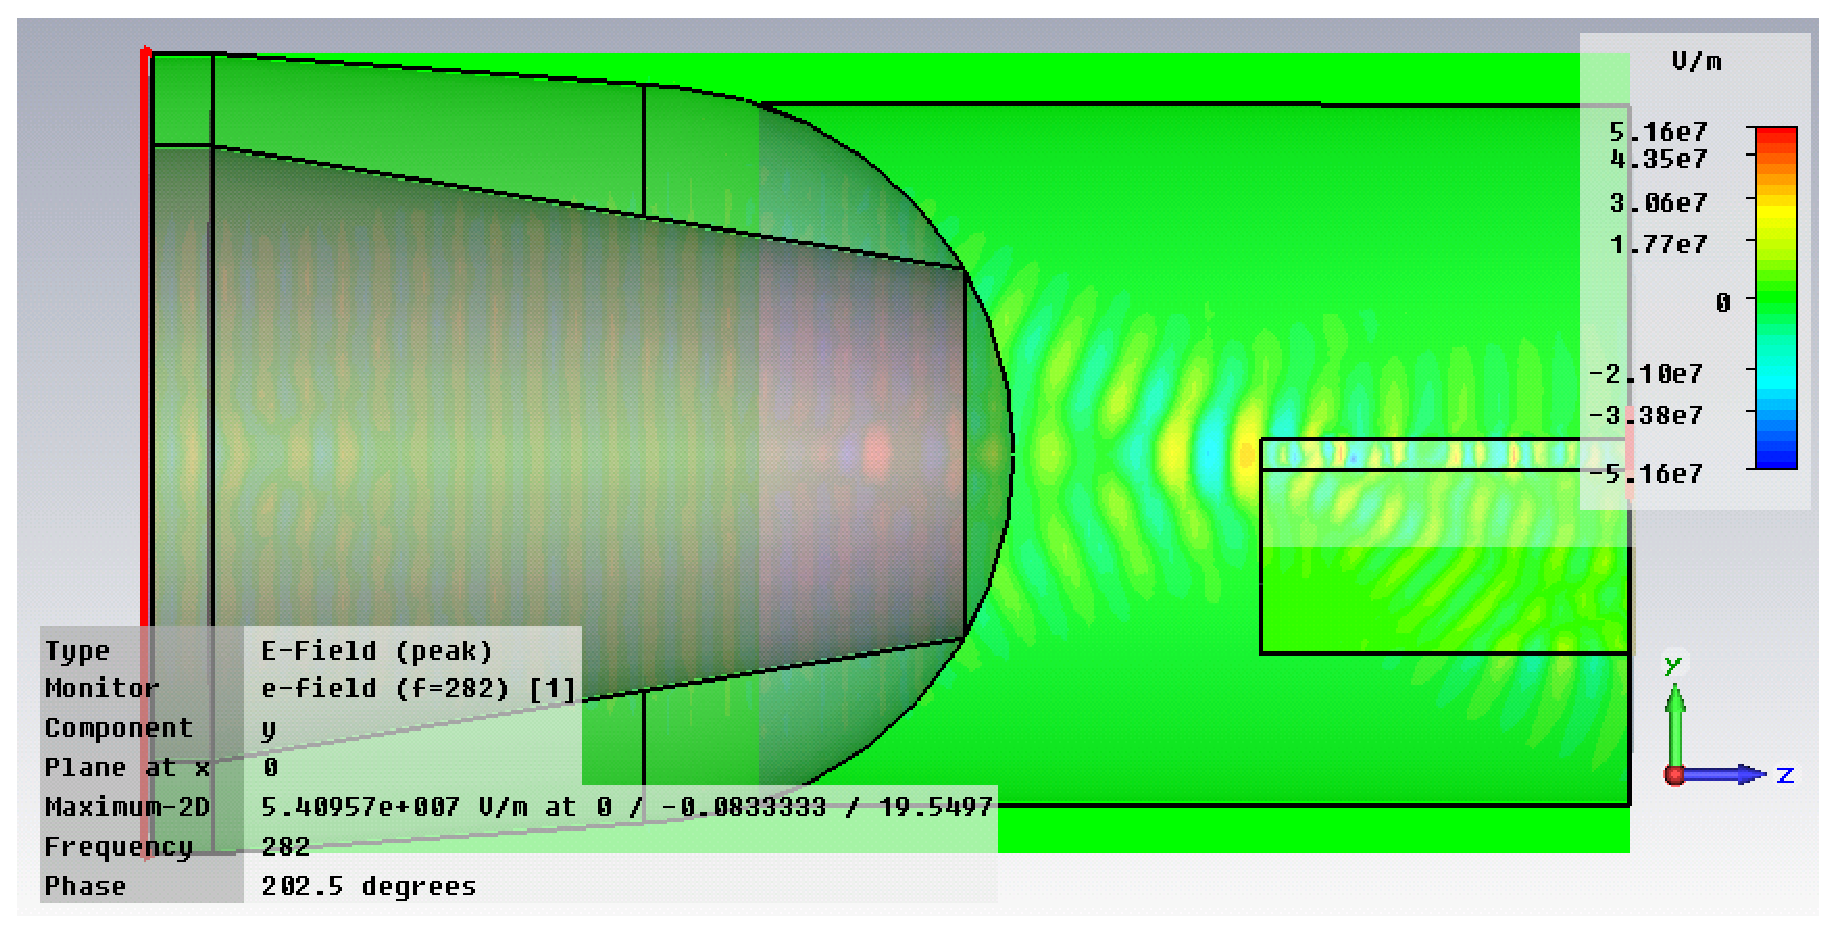
\includegraphics[width=0.5 \textwidth]{bilder/basic_waveguide_efield}
	\label{fig:coupling_e_field}
	\caption{E-Field demonstration by  coupling.}
\end{figure}
\begin{figure}
\centering
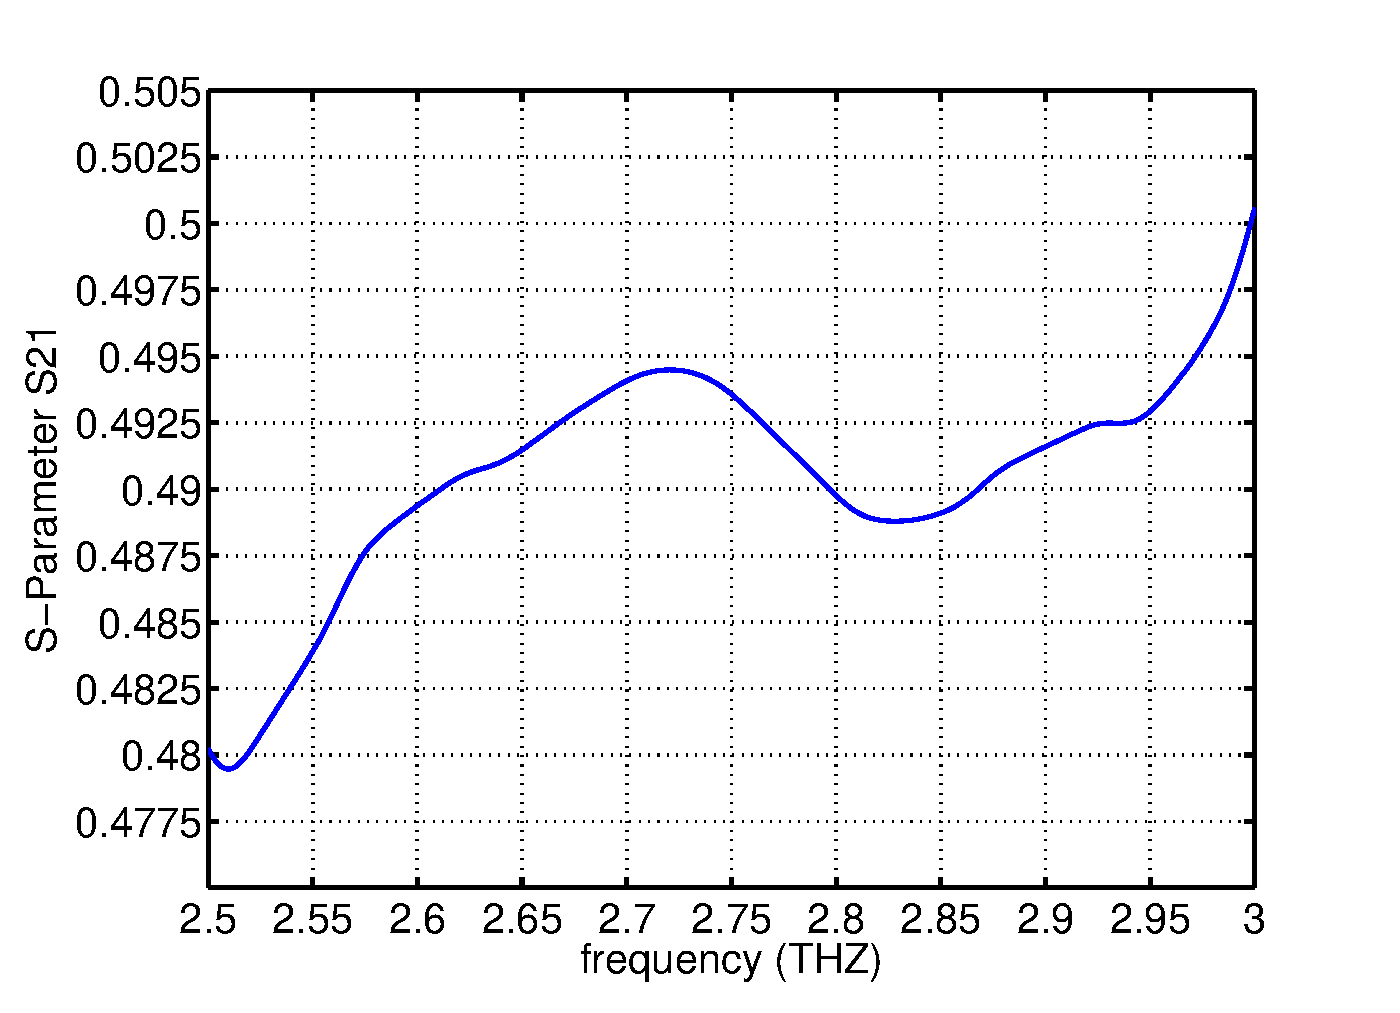
\includegraphics[width=0.7\textwidth]{bilder/original_coupling_efficiency}
\caption{coupling efficiency in Frequency area.}
\label{fig:orignial_coupling_efficiency}
\end{figure}

\begin{figure}[!ht]
\centering
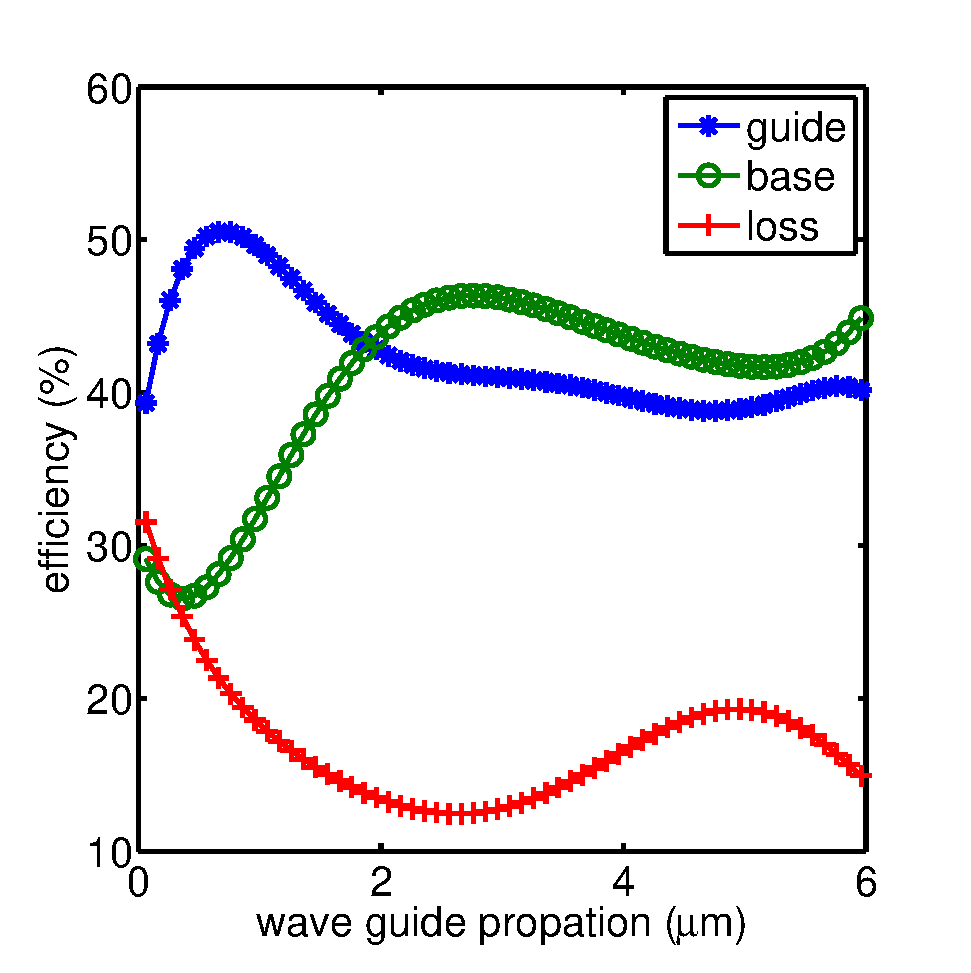
\includegraphics[width=0.7\textwidth]{bilder/power_distribution}
\caption{power distribution along the waveguide.}
\label{fig:power_distribution}
\end{figure}

